% --- UNIVERSAL PREAMBLE BLOCK ---
\documentclass[11pt, a4paper]{article}
\usepackage[a4paper, top=2.5cm, bottom=2.5cm, left=2cm, right=2cm]{geometry}
\usepackage[T1]{fontenc}
\usepackage[utf8]{inputenc}
\usepackage{lmodern}
\usepackage{amsmath}
\usepackage{array}
\usepackage{booktabs}
\usepackage{xcolor}
\usepackage{verbatim}
\usepackage{graphicx}
\graphicspath{{./}{../../graficos/}}
\usepackage{fancyhdr}
\usepackage{titlesec}
\usepackage{lastpage}
\usepackage[section]{placeins}
\usepackage[hidelinks]{hyperref}

\usepackage[spanish, es-tabla]{babel}

% Add because main language is not English
\usepackage{enumitem}
\setlist[itemize]{label=-}

% Professional Color Palette for Chaco For Ever (Gray/Teal/Red/Amber)
\definecolor{primary}{HTML}{0F172A}    % Dark Slate
\definecolor{alertred}{HTML}{DC2626}   % Red-600
\definecolor{accentgreen}{HTML}{0F766E}% Teal-700
\definecolor{warnamber}{HTML}{D97706}  % Amber-600
\definecolor{lightgray}{HTML}{F8FAFC}  % Slate-50
\definecolor{bordergray}{HTML}{E2E8F0} % Slate-200
\definecolor{darkgray}{HTML}{475569}   % Slate-600

% Custom styled frame box command for warnings
\newcommand{\alertbox}[2]{%
  \noindent\colorbox{lightgray}{%
    \parbox{\dimexpr\textwidth-2\fboxsep\relax}{%
      \raggedright
      \smallskip
      \textbf{\color{alertred}{#1}}\par\smallskip
      \small #2\par\smallskip
    }%
  }%
  \par\vspace{3mm}
}

% Custom command for green highlighting
\newcommand{\successbox}[2]{%
  \noindent\colorbox{lightgray}{%
    \parbox{\dimexpr\textwidth-2\fboxsep\relax}{%
      \raggedright
      \smallskip
      \textbf{\color{accentgreen}{#1}}\par\smallskip
      \small #2\par\smallskip
    }%
  }%
  \par\vspace{3mm}
}

% Colores de resaltado tipo marcador (highlighter)
\definecolor{markred}{HTML}{FEE2E2}    % rojo claro — dato negativo
\definecolor{markgreen}{HTML}{D1FAE5}  % verde claro — dato positivo
\definecolor{markamber}{HTML}{FEF3C7}  % ámbar claro — dato clave neutro

% Resaltados en línea (fondo tenue + negrita)
\newcommand{\mR}[1]{\textbf{#1}}
\newcommand{\mG}[1]{\textbf{#1}}
\newcommand{\mA}[1]{\textbf{#1}}

\setlength{\parindent}{0pt}
\setlength{\parskip}{6pt}

% --- Encabezado / pie de página ---
\pagestyle{fancy}
\fancyhf{}
\renewcommand{\headrulewidth}{0.4pt}
\renewcommand{\footrulewidth}{0.4pt}
\fancyhead[L]{\small\color{darkgray}\textsc{Chaco For Ever} $\bullet$ Informe de Partido}
\fancyhead[R]{\small\color{darkgray}Fecha 19 $\bullet$ 2026}
\fancyfoot[L]{\footnotesize\color{darkgray}Uso interno del Cuerpo Técnico}
\fancyfoot[R]{\footnotesize\color{darkgray}Página \thepage\ de \pageref{LastPage}}

% --- Estilo de secciones (regla de color debajo del título) ---
\titleformat{\section}
  {\normalfont\Large\bfseries\color{primary}}
  {\thesection}{0.6em}{}
  [\vspace{-2mm}\noindent{\color{accentgreen}\rule{\textwidth}{1.2pt}}]
\titlespacing*{\section}{0pt}{4mm}{4mm}

\titleformat{\subsection}
  {\normalfont\large\bfseries\color{darkgray}}
  {\thesubsection}{0.6em}{}
\titlespacing*{\subsection}{0pt}{3mm}{2mm}

\hypersetup{
  pdftitle={Informe de Partido -- Chaco For Ever vs Acassuso 2026},
  pdfauthor={Departamento de Big Data \& Análisis Táctico},
  pdfsubject={Fecha 19 -- Primera Nacional 2026},
}

\begin{document}

% --- HEADER BLOCK ---
\begin{center}
  \colorbox{primary}{%
    \parbox{\dimexpr\textwidth-2\fboxsep\relax}{%
      \vspace{4mm}
      \centering
      \color{white}
      \textsc{\Large Chaco For Ever} \\
      \smallskip
      \textbf{\Large INFORME DE PARTIDO} \\
      \vspace{1mm}
      \small Fecha 19 $\bullet$ Chaco For Ever 1 -- 1 Acassuso $\bullet$ Primera Nacional 2026
      \vspace{4mm}
    }%
  }
\end{center}

\vspace{4mm}

% --- METADATA ---
\begin{tabular}{ll}
  \textbf{Destinatarios:} & Cuerpo Técnico, Comisión Directiva \\
  \textbf{Creadores:} & Cordeiro Mariano Angel y Casco Tobias \\
  \textbf{Contacto:} & cordeiromariano17@gmail.com \\
  \textbf{Partido:} & Chaco For Ever 1 -- 1 Acassuso (local, entretiempo 1-0) \\
  \textbf{Goles:} & Matías Romero (26') \quad / \quad A. Hermoso (56') \\
  \textbf{Alcance del Análisis:} & Fecha 19, leída con las herramientas de la temporada 2026 \\
\end{tabular}

\vspace{4mm}
\hrule
\vspace{4mm}

% --- SECCIÓN 1: QUÉ PASÓ EN EL PARTIDO ---
\section*{1. Qué Pasó en el Partido}

Chaco jugó bien y empato en casa. Fue el equipo que más tuvo la pelota, el que más pateó y el que abrió el marcador con un gol de Matías Romero. Y aun así terminó empatado. Acassuso lo igualó con la única pelota clara que se le presentó en todo el partido, y encima la metió en el peor momento posible: apenas arrancó el segundo tiempo, que viene siendo el punto flojo del equipo toda la temporada.

En el informe vas a ver la sigla \textbf{xG}. Es una forma sencilla de medir qué tan clara fue una situación de gol: un valor cercano a 1 es un gol casi hecho, y uno cercano a 0 es un remate muy difícil. Sumando el xG de un equipo se ve cuánto peligro generó en total, más allá de si la embocó o no.

\begin{table}[h!]
  \centering
  \caption{Cómo quedaron los números del partido (Chaco / Acassuso)}
  \vspace{2mm}
  \begin{tabular}{lll}
    \toprule
    \textbf{} & \textbf{Chaco} & \textbf{Acassuso} \\
    \midrule
    Goles & \mA{1} (Romero 26') & \mA{1} (Hermoso 56') \\
    Tuvo la pelota & \mG{58\%} & 42\% \\
    Peligro generado (xG) & \mG{1.86} & 1.22 \\
    Remates (al arco) & \mG{16 (6)} & 10 (4) \\
    Córners & 7 & 5 \\
    Pases (bien dados) & 367 (241) & 285 (172) \\
    Amarillas & 3 & 3 \\
    \bottomrule
  \end{tabular}
\end{table}

\alertbox{El partido en dos líneas}{Chaco fue más peligroso por juego y por cantidad: generó más chances claras ($1.86$ de xG contra $1.22$) y pateó 16 veces contra 10. Perdió dos puntos por lo mismo de siempre: no supo cuidar la ventaja y se le complicó el partido justo al arranque del segundo tiempo. No jugó mal. Le volvió a pasar lo que ya le venía pasando.}

% --- GRÁFICO 1: xG por tramos ---
\begin{figure}[htbp]
  \centering
  \fbox{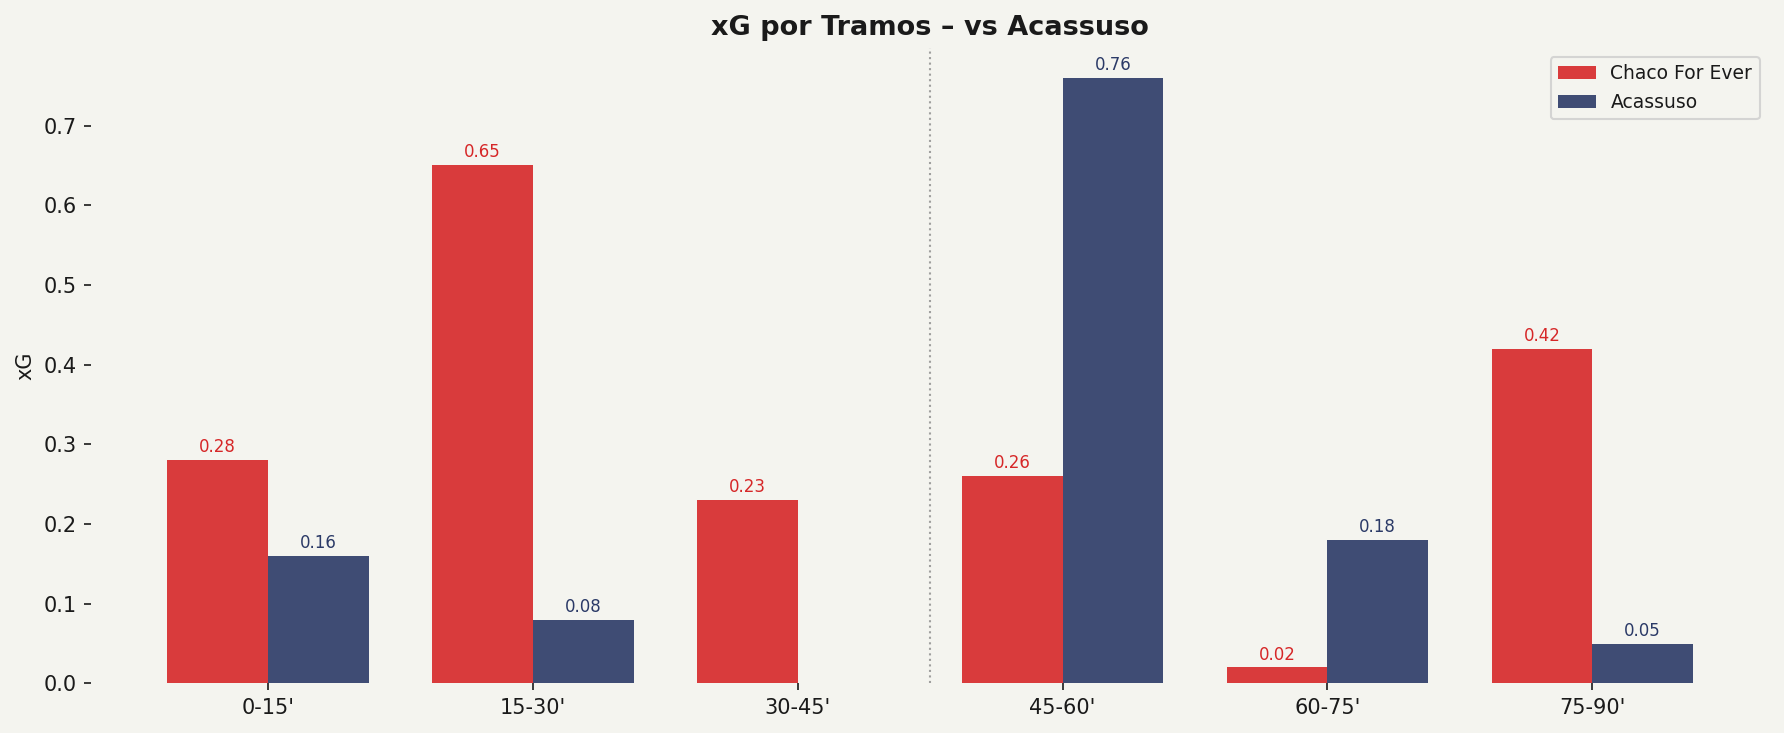
\includegraphics[width=0.98\textwidth]{xg_tramos.png}}
  \caption{El partido dividido en tramos de 15 minutos, según el peligro que generó cada equipo. Chaco (rojo) fue más peligroso en cinco de los seis tramos. El único donde Acassuso lo superó, y por mucho ($0.76$ a $0.26$), es el del 45 al 60: justo el ratito en el que llegó el empate.}
  \label{fig:xg_tramos}
\end{figure}

% --- SECCIÓN 2: LO QUE YA SABÍAMOS ---
\section*{2. Lo Que Ya Sabíamos, y Volvió a Pasar}

Hace varias fechas que venimos siguiendo dos problemas que a Chaco se le repiten partido tras partido. Contra Acassuso aparecieron los dos, juntos, en el mismo partido.

\subsection*{Se pone en ventaja, pero no la sostiene}
Ya había pasado tres veces en la temporada: Chaco se ponía 1-0 y no lograba mantenerlo. Contra Acassuso fue la \mR{cuarta}. Se fue al descanso ganando \mA{1-0}, manejando el partido, y terminó \mR{1-1}. Ponerse arriba no es el problema, lo hace seguido. El problema es lo que viene después del gol.

\subsection*{El bajón al arranque del segundo tiempo}
Si uno mira en qué minutos le hacen los goles a Chaco durante todo el año, hay una franja que se despega de todas: entre el minuto \mR{45 y el 60}, apenas empieza el complemento. Hermoso empató justo ahí, al \mR{56'}. Con ese gol, esa franja ya suma \mR{9 goles en contra} en la temporada. Más de un tercio (el \mR{36\%}) de todos los goles que le hicieron a Chaco en el año caen en esos quince minutos.

Este partido lo mostró casi de manual. De todo el peligro que generó Acassuso en los 90 minutos, \mR{más de la mitad} salió de esa sola franja de 45 a 60. En el resto del partido casi no inquietó. Fue el único ratito en que fue superior, y le alcanzó para empatar.

\alertbox{El mismo guion, en un solo partido}{Lo que la temporada muestra fecha tras fecha, este partido lo repitió en chiquito. Acassuso no fue mejor que Chaco. Solo apareció en el momento justo en que el equipo se relaja al salir del vestuario. Es algo bien concreto para trabajar: cómo arranca Chaco el segundo tiempo.}

% --- GRÁFICO 2: momentum ---
\begin{figure}[htbp]
  \centering
  \fbox{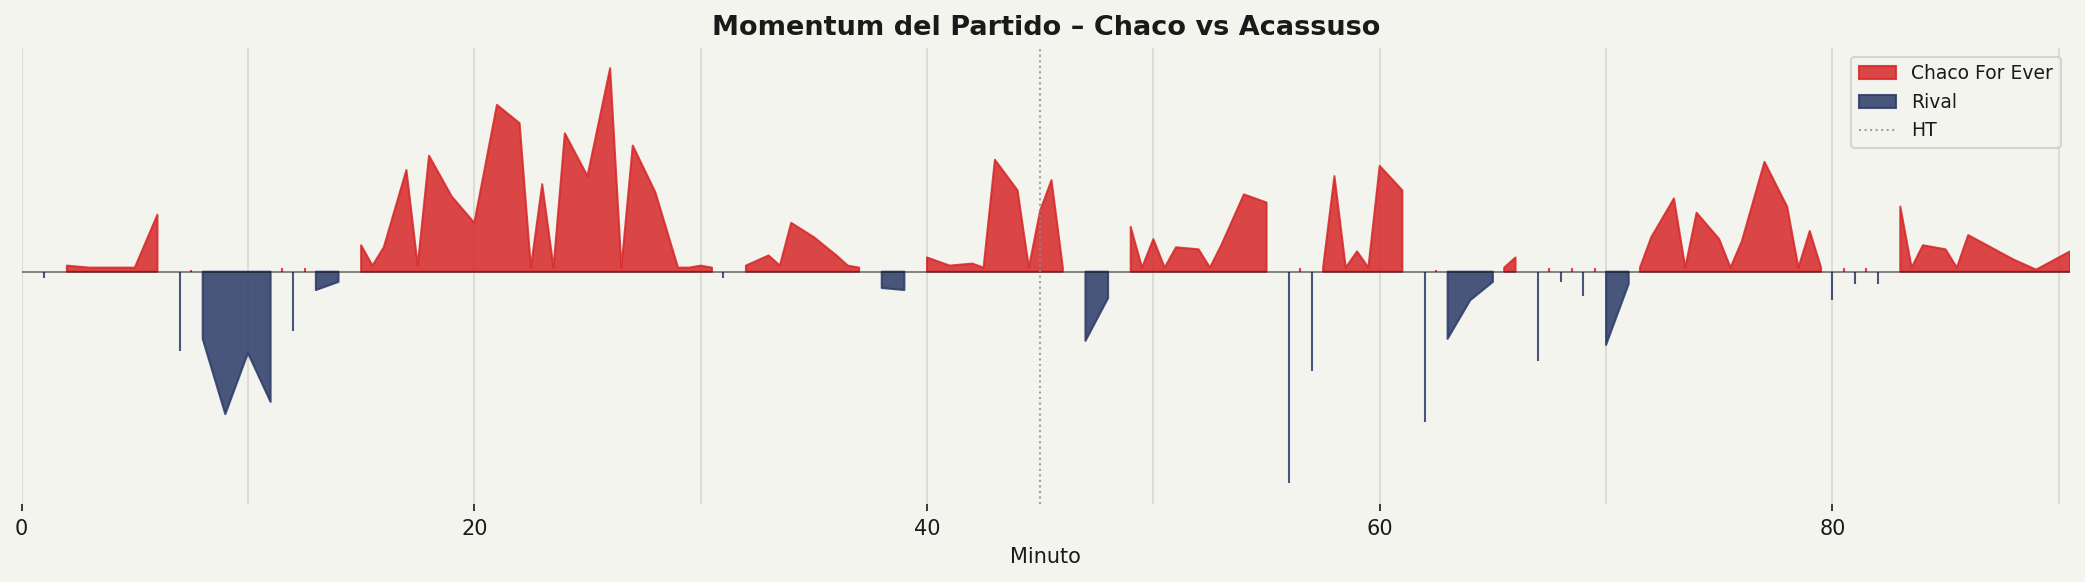
\includegraphics[width=0.98\textwidth]{momentum.png}}
  \caption{El pulso del partido minuto a minuto. Cuanto más grande la ola roja, más cerca estuvo Chaco del arco rival; la azul es Acassuso. El dominio de Chaco es casi permanente, con su pico en el 15-30 donde llegó el gol de Romero. El empate al 56' cae en uno de los poquitos avances de Acassuso de todo el segundo tiempo.}
  \label{fig:momentum}
\end{figure}

% --- SECCIÓN 3: ROMERO ---
\section*{3. Romero: la Vuelta con Gol}

El que volvió y desmostro fue \mG{Matías Romero}. A los 26 minutos ganó de cabeza dentro del área y puso el 1-0, en su vuelta a Chaco. Terminó como \mG{la figura de la cancha}, con la mejor nota del partido ($8.1$), y fue lejos el más peligroso de los once.

\successbox{La vuelta soñada}{Romero no solo hizo el gol. Fue el que llevó adelante casi todo el ataque de Chaco: él solo generó \mG{la mitad del peligro} de todo el equipo. Remató tres veces al arco, tuvo un disparo desde fuera del area al 60' que le tapó el arquero y dos cabezazos más que pasaron cerca. Y ganó \mG{11 de los 15 duelos aéreos} que disputó: por arriba, no lo pudo parar nadie.}

Al lado, el otro refuerzo que fue titular, \mG{Leandro Fernández}, fue el que más ayudó a generar juego por afuera: metió cinco centros buenos al área y tres pases clave, de esos que dejan a un compañero de cara al gol. Las dos caras nuevas del plantel se hicieron notar desde el arranque.

% --- GRÁFICO 3: ratings ---
\begin{figure}[htbp]
  \centering
  \fbox{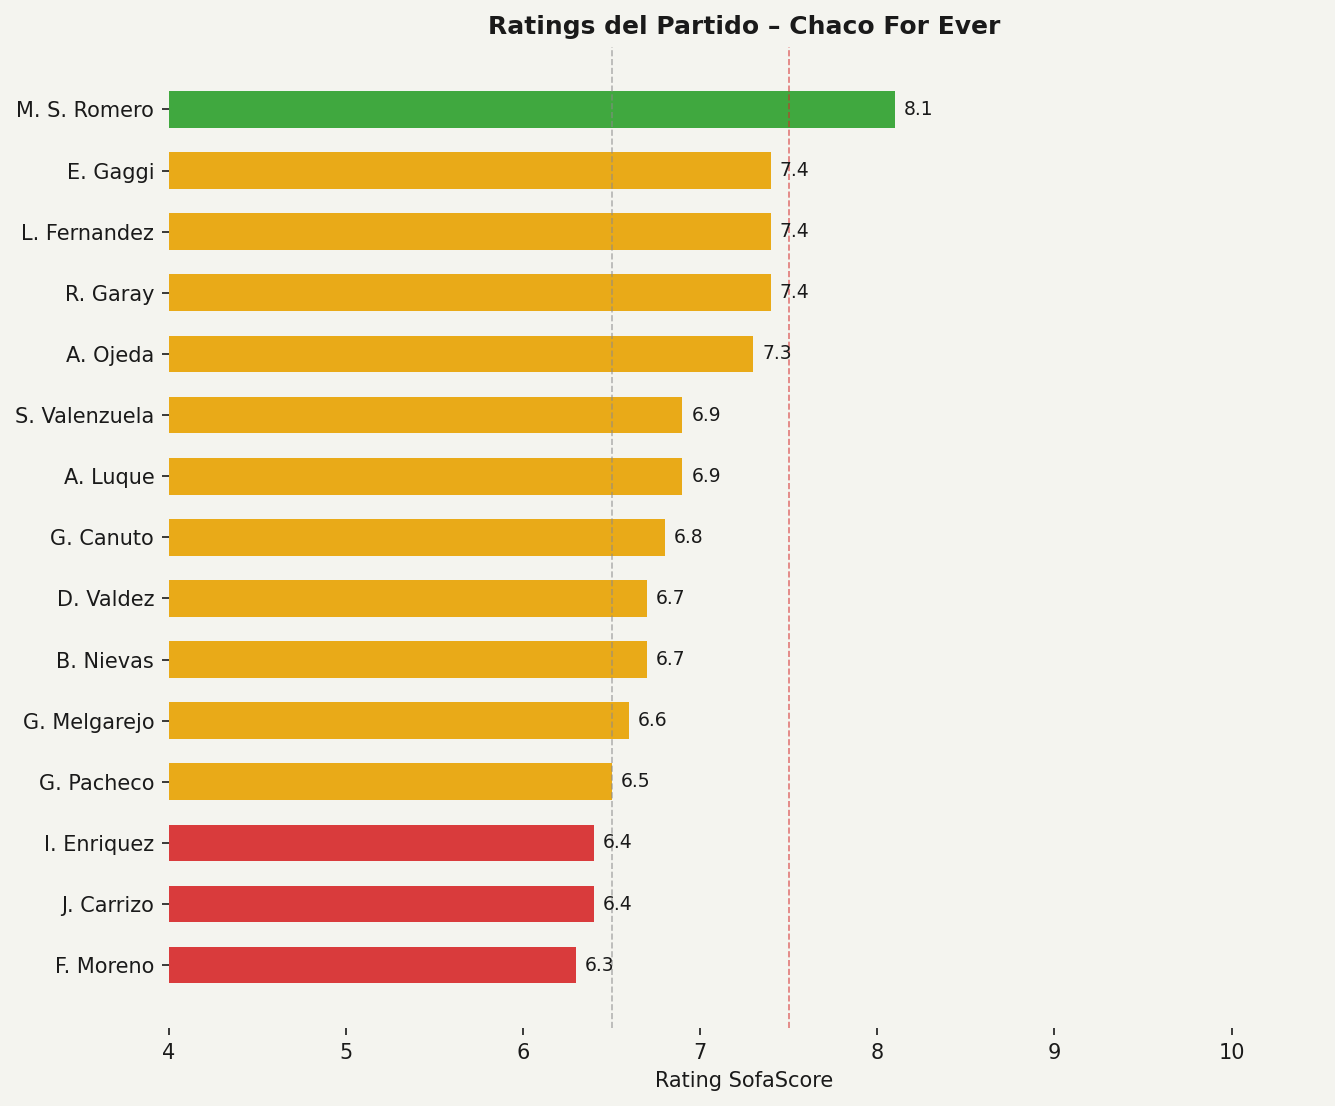
\includegraphics[width=0.90\textwidth]{ratings_jugadores.png}}
  \caption{Las notas de los jugadores. Romero arriba de todo con 8.1, seguido por Gaggi, Garay y Fernández con 7.4. El juego de ataque pasó por los dos refuerzos.}
  \label{fig:ratings}
\end{figure}

% --- SECCIÓN 4: DATOS PARA TENER EN CUENTA ---
\section*{4. Datos Para Tener en Cuenta}

\subsection*{Detalles que dejó el partido}
\begin{itemize}
  \item \textbf{Acassuso se paró a aguantar.} Rechazó \mA{43 pelotas} y cortó otras \mA{17}, contra 13 y 8 de Chaco. Se replegó, despejó y esperó su momento. Su gol no salió de un ataque elaborado, salió de la única jugada clara que le quedó.

    \begin{figure}[htbp]
    \centering
    \fbox{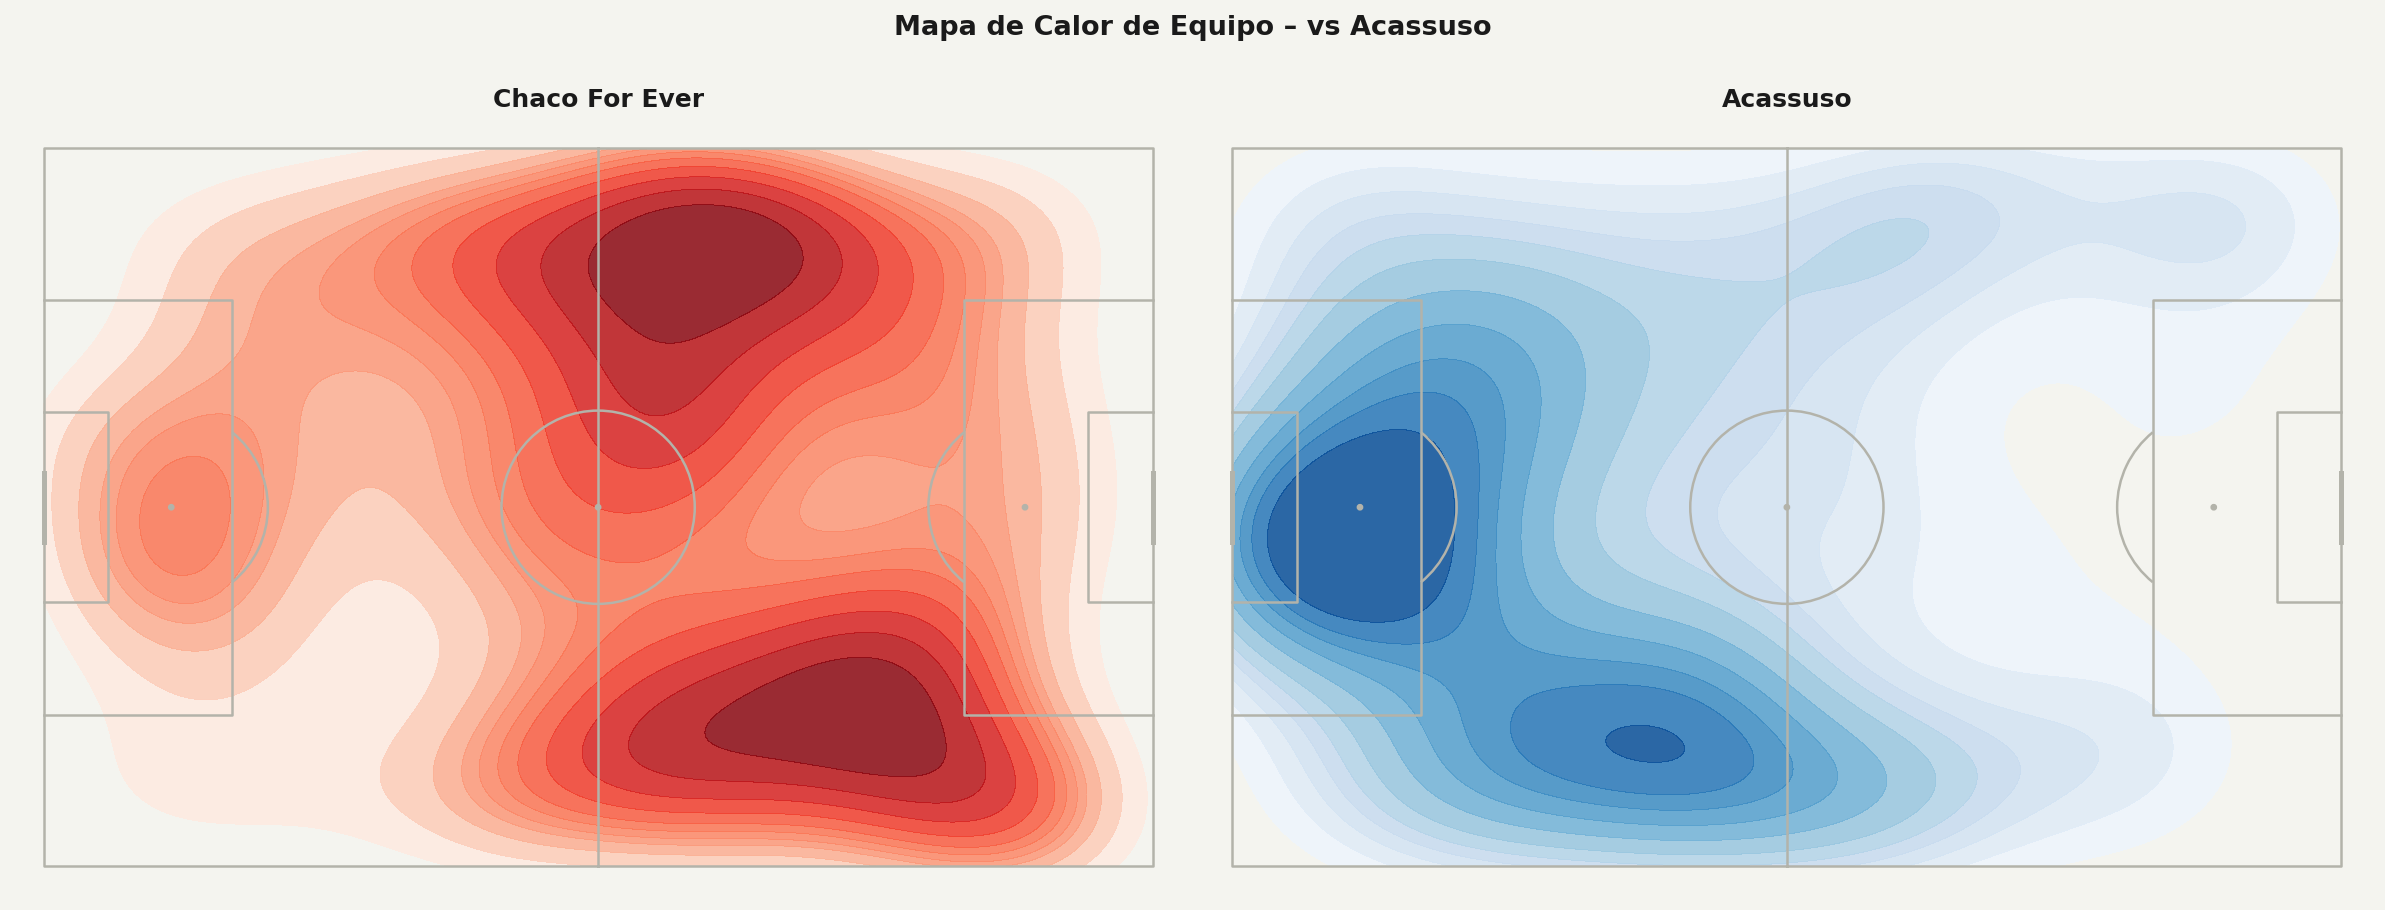
\includegraphics[width=0.7\textwidth]{heatmap_equipo.png}}
    \caption{En el Mapa de Calor podemos observar cómo en este partido Chaco tomó una posición más ofensiva y forzó un repliegue defensivo en Acassuso.}
    \label{fig:heatmap}
    \end{figure}

  \item \textbf{No metió ni un centro.} Acassuso probó \mR{nueve centros} al área y no le llegó ninguno a un compañero. Todo su peligro pasó por el medio, en esa única jugada.
  \item \textbf{Romero fue medio equipo.} El peligro que generó él solo fue prácticamente igual al de todos sus compañeros sumados.
  \item \textbf{El córner y pelota parada, otra materia pendiente.} Chaco tiró \mR{siete córners} y no convirtió ninguno, con cabezazos de Romero (58') y un tiro libre que llego a Garay (24') que no entraron. Se repite todo el año: el equipo es bueno por arriba, pero todavía no le saca jugo a la pelota parada.
\end{itemize}

\subsection*{Para el cuerpo técnico}
\begin{itemize}
  \item \textbf{El partido confirma lo que ya veníamos viendo.} El nivel de juego alcanza. Lo que falla es cuidar la ventaja y arrancar bien el segundo tiempo. Dos cosas puntuales para trabajar en la semana, porque para generar, el equipo genera.
  \item \textbf{El arranque del complemento.} Con el empate al 56' ya son nueve goles en contra en esa franja en el año. Vale la pena una rutina para salir metidos del vestuario y mirar en video esos primeros diez minutos.
  \item \textbf{Romero y Fernández, para seguir apostando.} Los dos refuerzos rindieron en su debut. Romero además le da el gol y la referencia de área al equipo.
  \item \textbf{Falta definir.} Chaco fue capaz de generar en ofensiva, pero el problema pasa por no sostener la ventaja. Especialmente con la inclusión de Romero, el equipo mejoró.
\end{itemize}

\end{document}
